\documentclass[12pt]{article}
\usepackage{amsmath}
\usepackage{geometry}
\usepackage{setspace}
\usepackage{graphicx}
\usepackage{fancyhdr}
\usepackage{xcolor}
\usepackage{titlesec}
\usepackage{booktabs}
\geometry{a4paper, margin=1in}
\setlength{\parindent}{0pt}
\setstretch{1.5}

% Header and Footer
\pagestyle{fancy}
\fancyhf{}
\fancyhead[L]{\textbf{19-AIBM4}} % Top-left text
\fancyhead[C]{\rule{\textwidth}{0.5pt}} % Top horizontal line
\fancyfoot[C]{\rule{\textwidth}{0.5pt}} % Bottom horizontal line
\fancyfoot[R]{\thepage} % Page number on the right

% Title formatting with red section headers
\titleformat{\section}[block]
  {\large\bfseries\sffamily\color{red}}
  {\thesection.}{1em}{}

\titleformat{\subsection}[block]
  {\normalsize\bfseries\sffamily\color{red}}
  {\thesubsection}{1em}{}

% Document content
\begin{document}

% -------------------------------------------------------------
% COVER PAGE
% -------------------------------------------------------------
\begin{titlepage}
\centering
% University logo or other image

\includegraphics[width=0.4\textwidth]{UoD_Engineering.jpg} \\
\vspace{20mm}

% Title and subtitle
{\LARGE \textbf{Feasibility Report for 19-AIBM4 Autonomous Material Mover}} \\[10pt]

\vspace{5mm}\hrule\vspace{15mm}

% Insert image with caption for the material mover
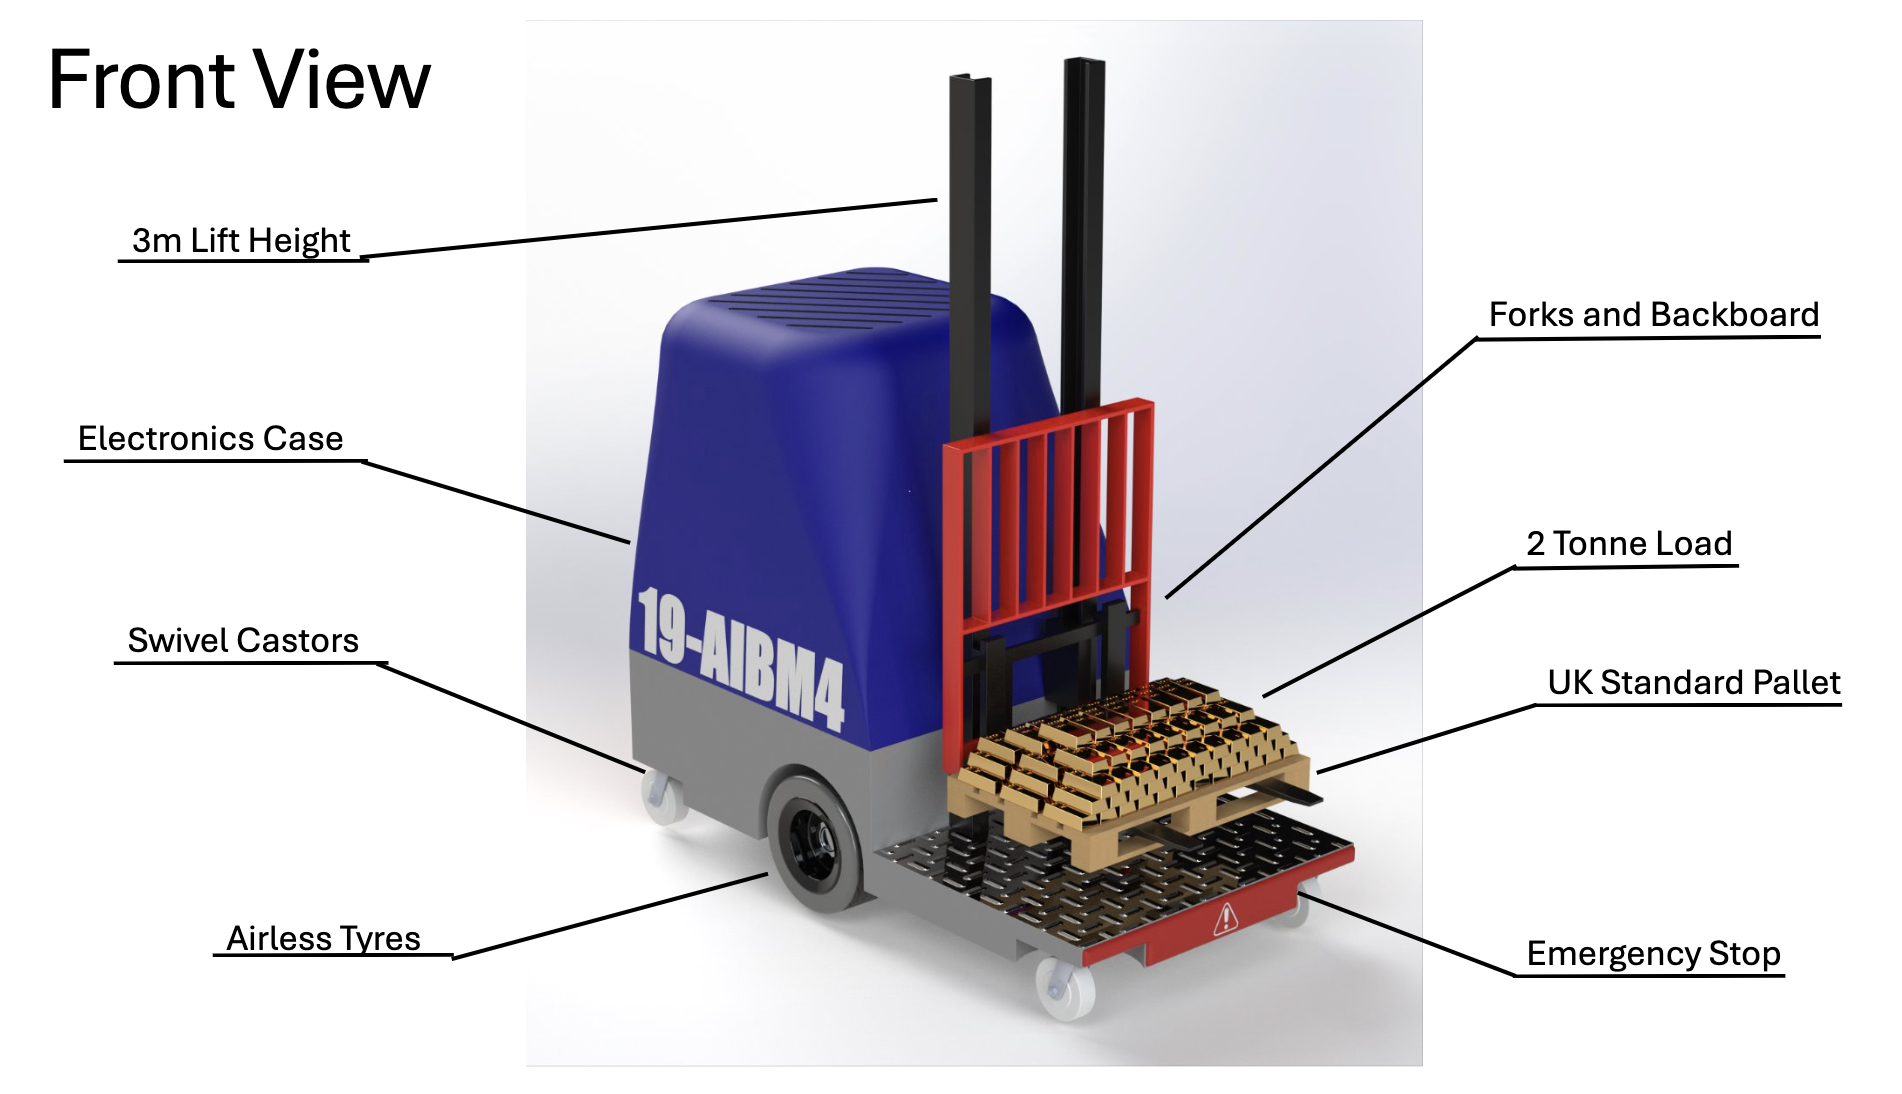
\includegraphics[width=0.8\textwidth]{Screenshot 2024-11-14 at 17.52.59.png}  \\  
\vspace{5mm}
\textit{Figure: Front View of the 19-AIBM4 Autonomous Material Mover} \\

\vspace{20mm}

% Title and author block
{\large \textbf{Co-first authors alphabetical-order}: Abi Wright, Anna Wigmore, Henry Billing, Jiaxi Wang, Louis Nangle, Will Woodward} \\ \vspace{2mm}
{Supervisor: Aissa Ikhlef, Bill Maxwell} \\[10pt]
{\small The University of Durham \\ \today}
\end{titlepage}

% -------------------------------------------------------------
% FRONTMATTER
% -------------------------------------------------------------
\tableofcontents
\newpage

% -------------------------------------------------------------
% MAIN CONTENT
% -------------------------------------------------------------

\section{Problem Statement}
Efficient, automated material handling within industrial environments is critical for the fourth industrial revolution. However, one area still heavily reliant on manual labor is transporting heavy materials between supplier delivery, storage, and production areas. This design project addresses these challenges by developing an automated material mover capable of transporting up to two tonnes of load within a factory setting.


\section{Introduction and Project Scope}
The estimated budget for this project is £60,000, covering labor, material mover parts, wiring, software, and programming.


\begin{figure}[h!]
    \centering
    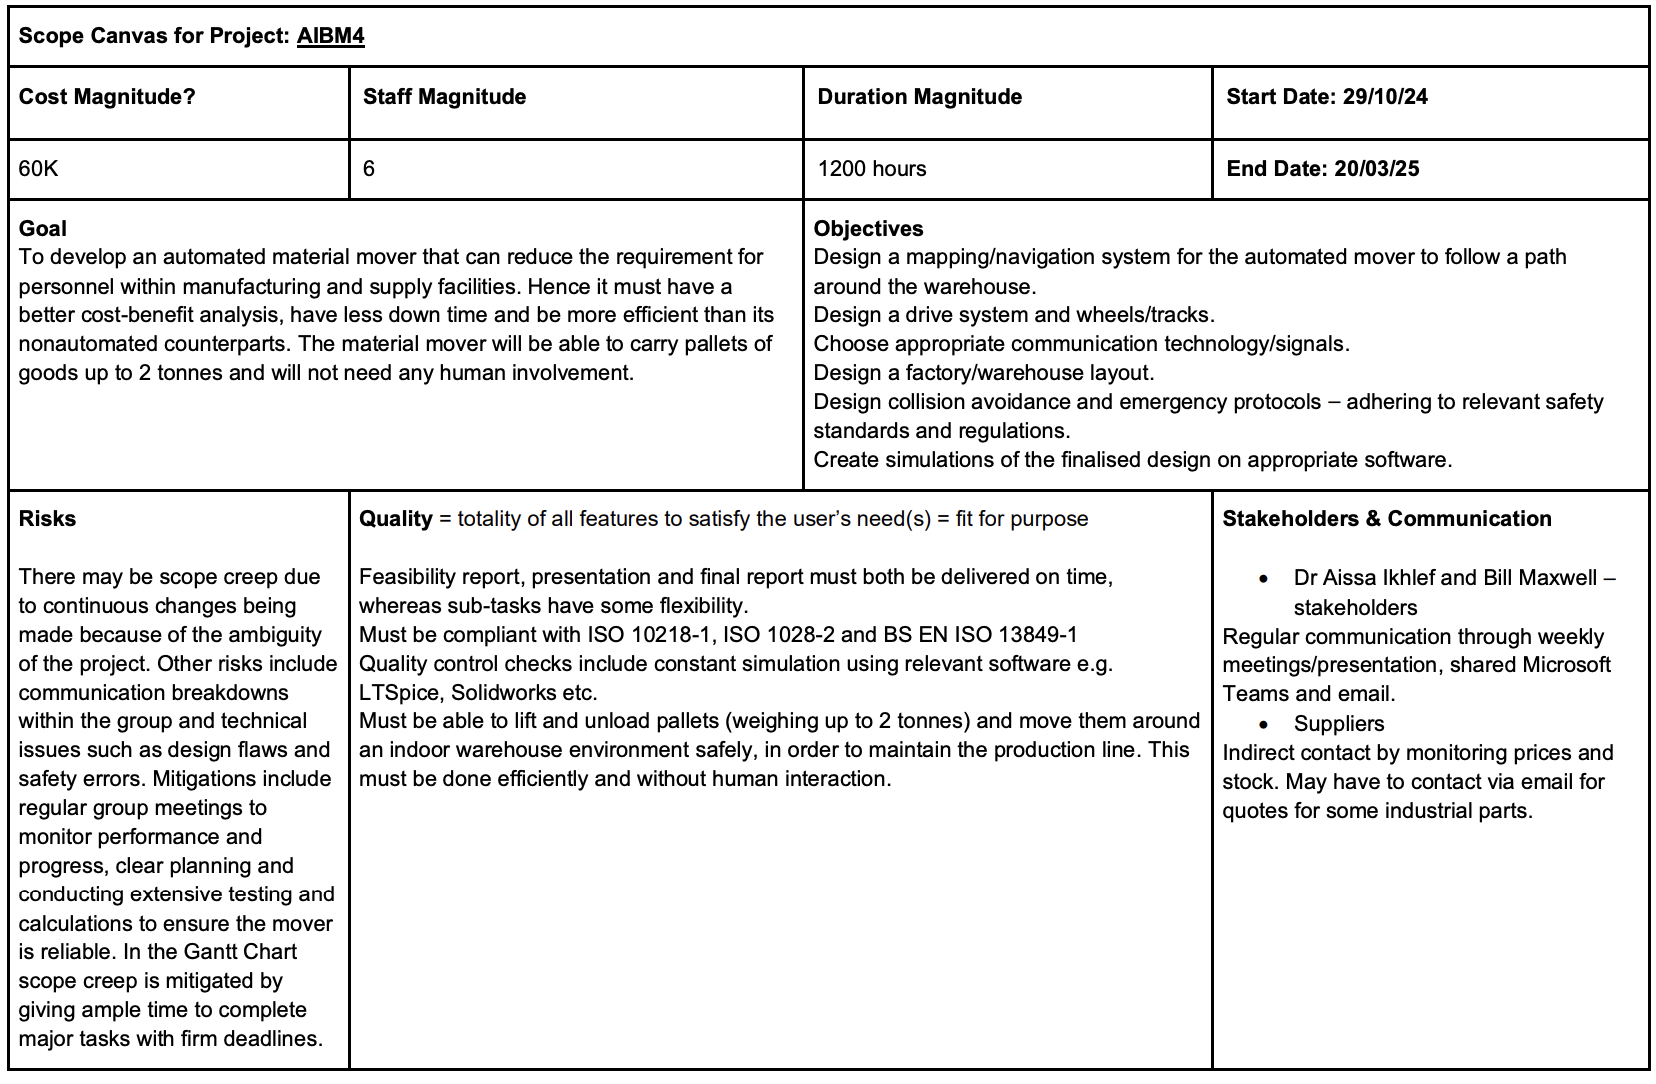
\includegraphics[width=1\textwidth]{scope1.png}
  \label{fig:Project Scope Document for AIBM4}
\end{figure}

\begin{figure}[h!]
    \centering
     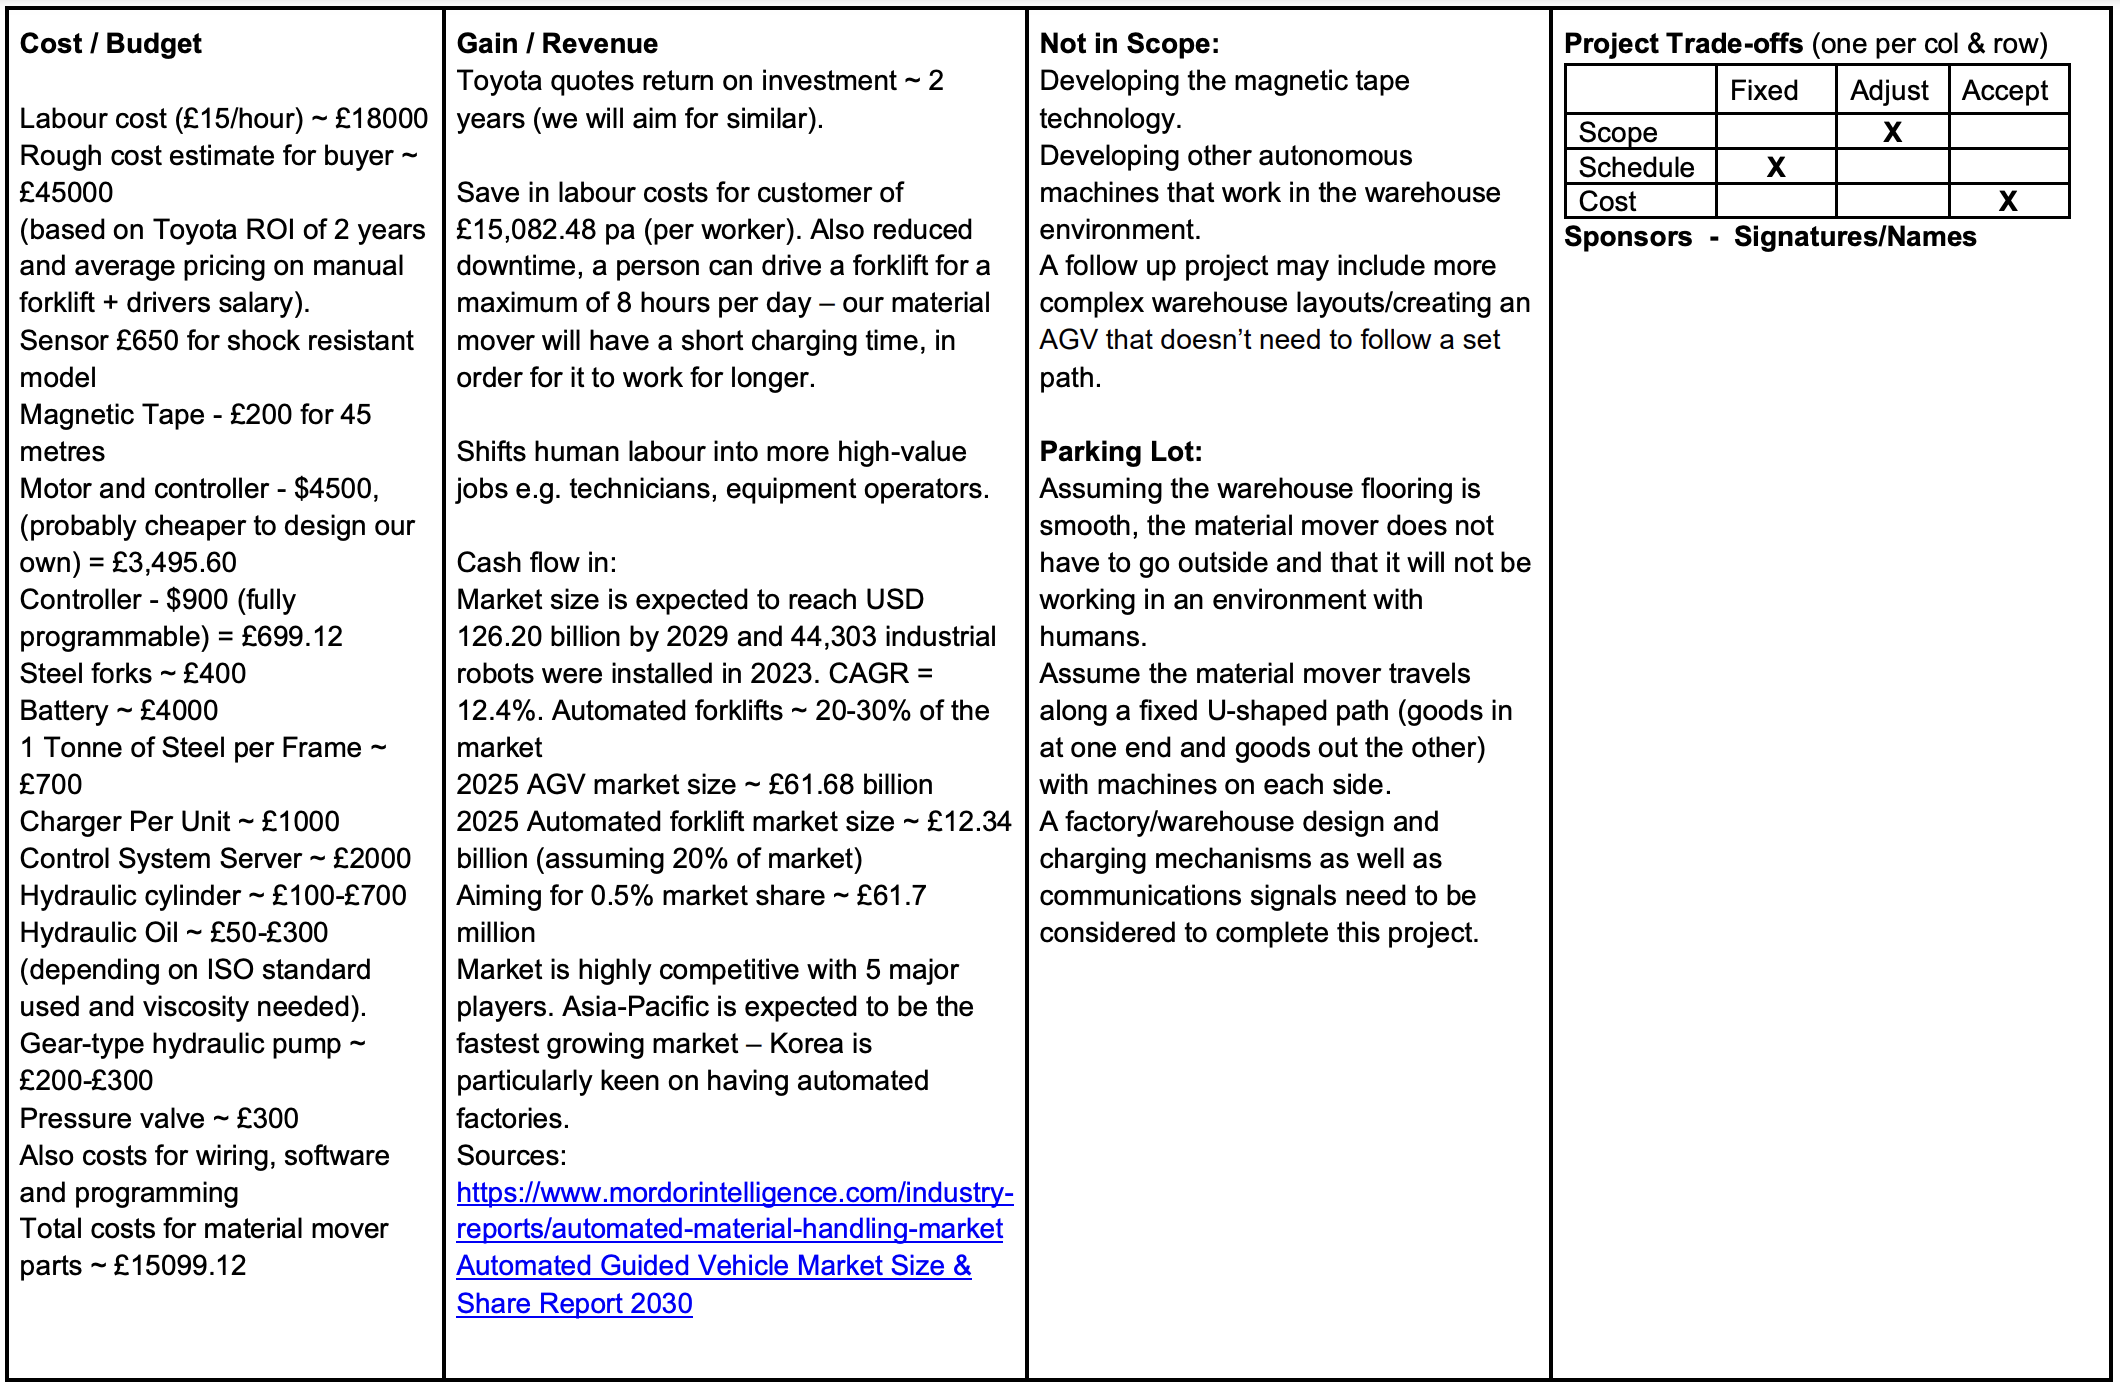
\includegraphics[width=1\textwidth]{scope2.png}
        \caption{Detailed Scope, Objectives, and Resources for Project AIBM4, focused on developing an automated material mover to enhance efficiency in manufacturing and supply facilities.}
         \label{fig:Project Scope Document for AIBM4}
\end{figure}



\newpage

\section{Concepts and Designs}
\subsection{Proposed Designs}
\begin{figure}[h!]
    \centering
    \includegraphics[width=0.9\textwidth]{design.png}
    \caption{Proposed Design Concepts}
\end{figure}

\subsection{Factory Layout}
\begin{figure}[h!]
    \centering
    \includegraphics[width=0.9\textwidth]{factory_layout.png}
    \caption{Factory Layout Integration}
\end{figure}

\newpage

\section{Strengths and Weaknesses of Concepts}
\begin{figure}[h!]
    \centering
    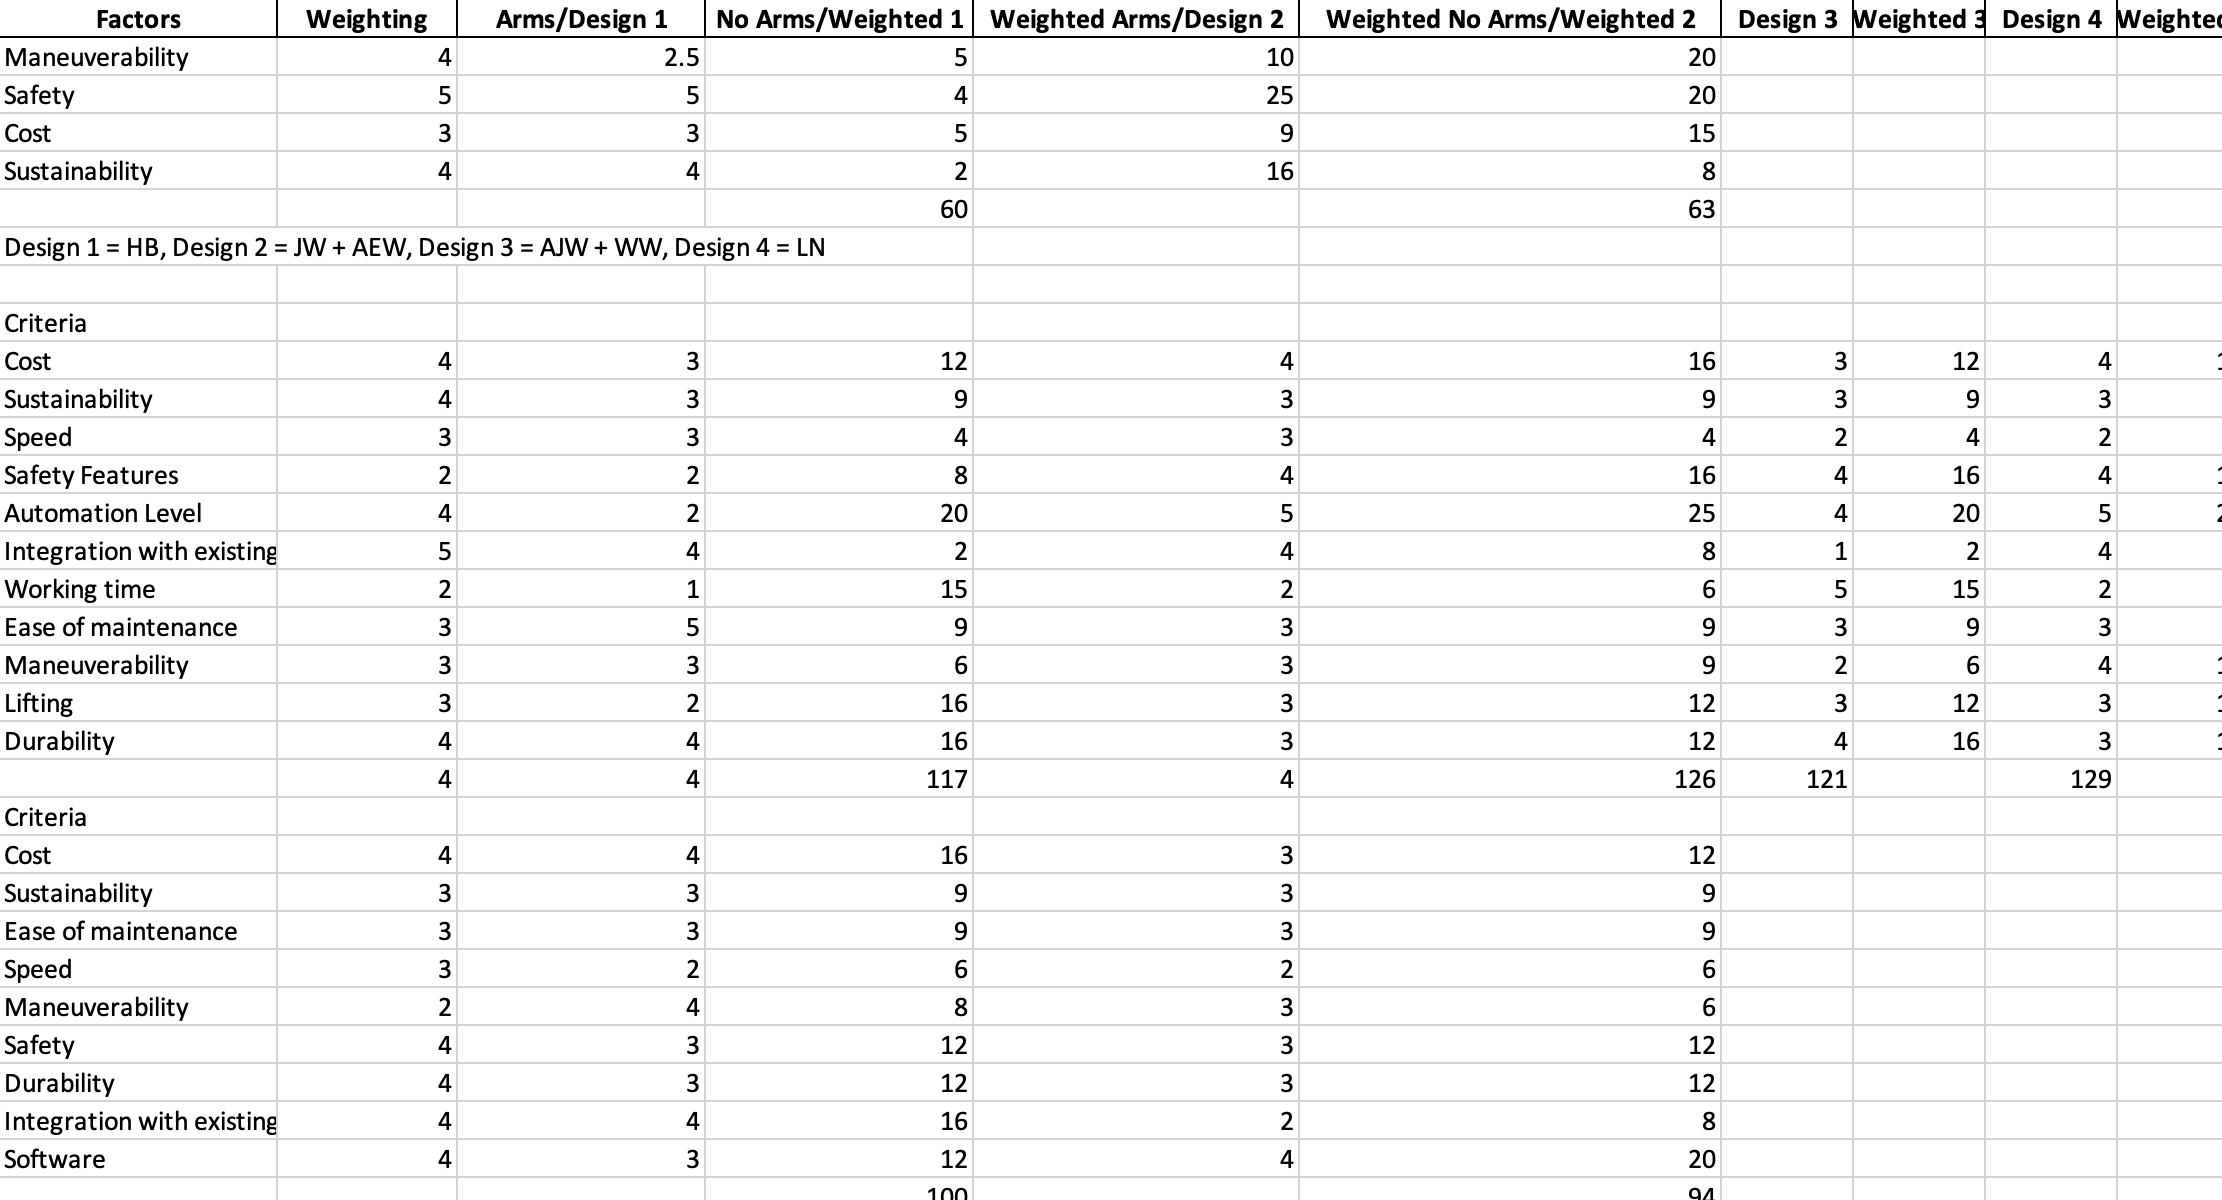
\includegraphics[width=0.9\textwidth]{matrix.png}
    \caption{Concept Evaluation Matrix}
\end{figure}

\begin{figure}[h!]
    \centering
    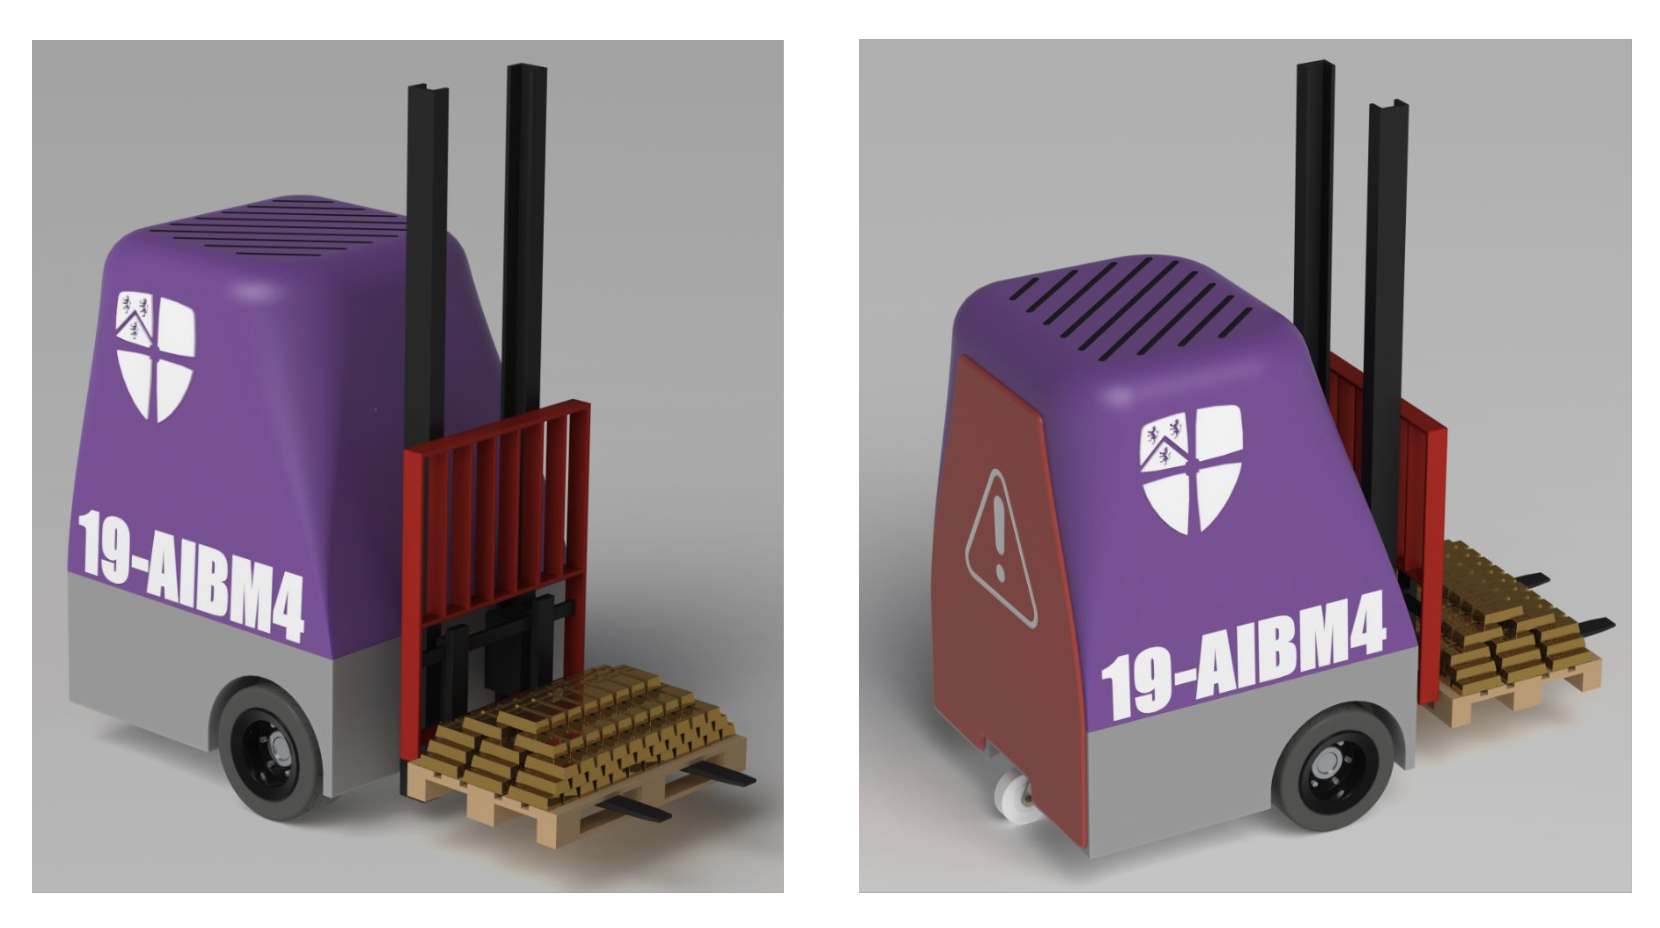
\includegraphics[width=0.9\textwidth]{finaldesign.png}
    \caption{finalized design}
\end{figure}


\section{Project Schedule}
Summarize your group’s timeline:
\begin{figure}[h!]
    \centering
    \includegraphics[width=0.9\textwidth]{gantt_chart.pdf}
    \caption{Project Gantt Chart}
\end{figure}

\newpage

\section{Expected Product Cost}
\begin{itemize}
    \item \textbf{Labor Costs:} £18,000
    \item \textbf{Material Costs:} £15,099.12
    \item \textbf{Overheads:} £10,000
    \item \textbf{Software and Simulation:} £2,000
    \item \textbf{Contingency:} £4,900.88
\end{itemize}
\textbf{Total Estimated Cost: £60,000}

\newpage

\section{Commercial Business Case}
\subsection{Financial Analysis}
\textbf{Revenue Potential:} The automated forklift market is projected to reach £12.34 billion by 2025. Achieving 0.5\% market share results in revenue of £61.7 million.

\textbf{Labor Savings:} Automating pallet movement saves approximately £15,082.48 per year per worker.

\newpage

% Include the image
\begin{figure}[h!]
    \centering
    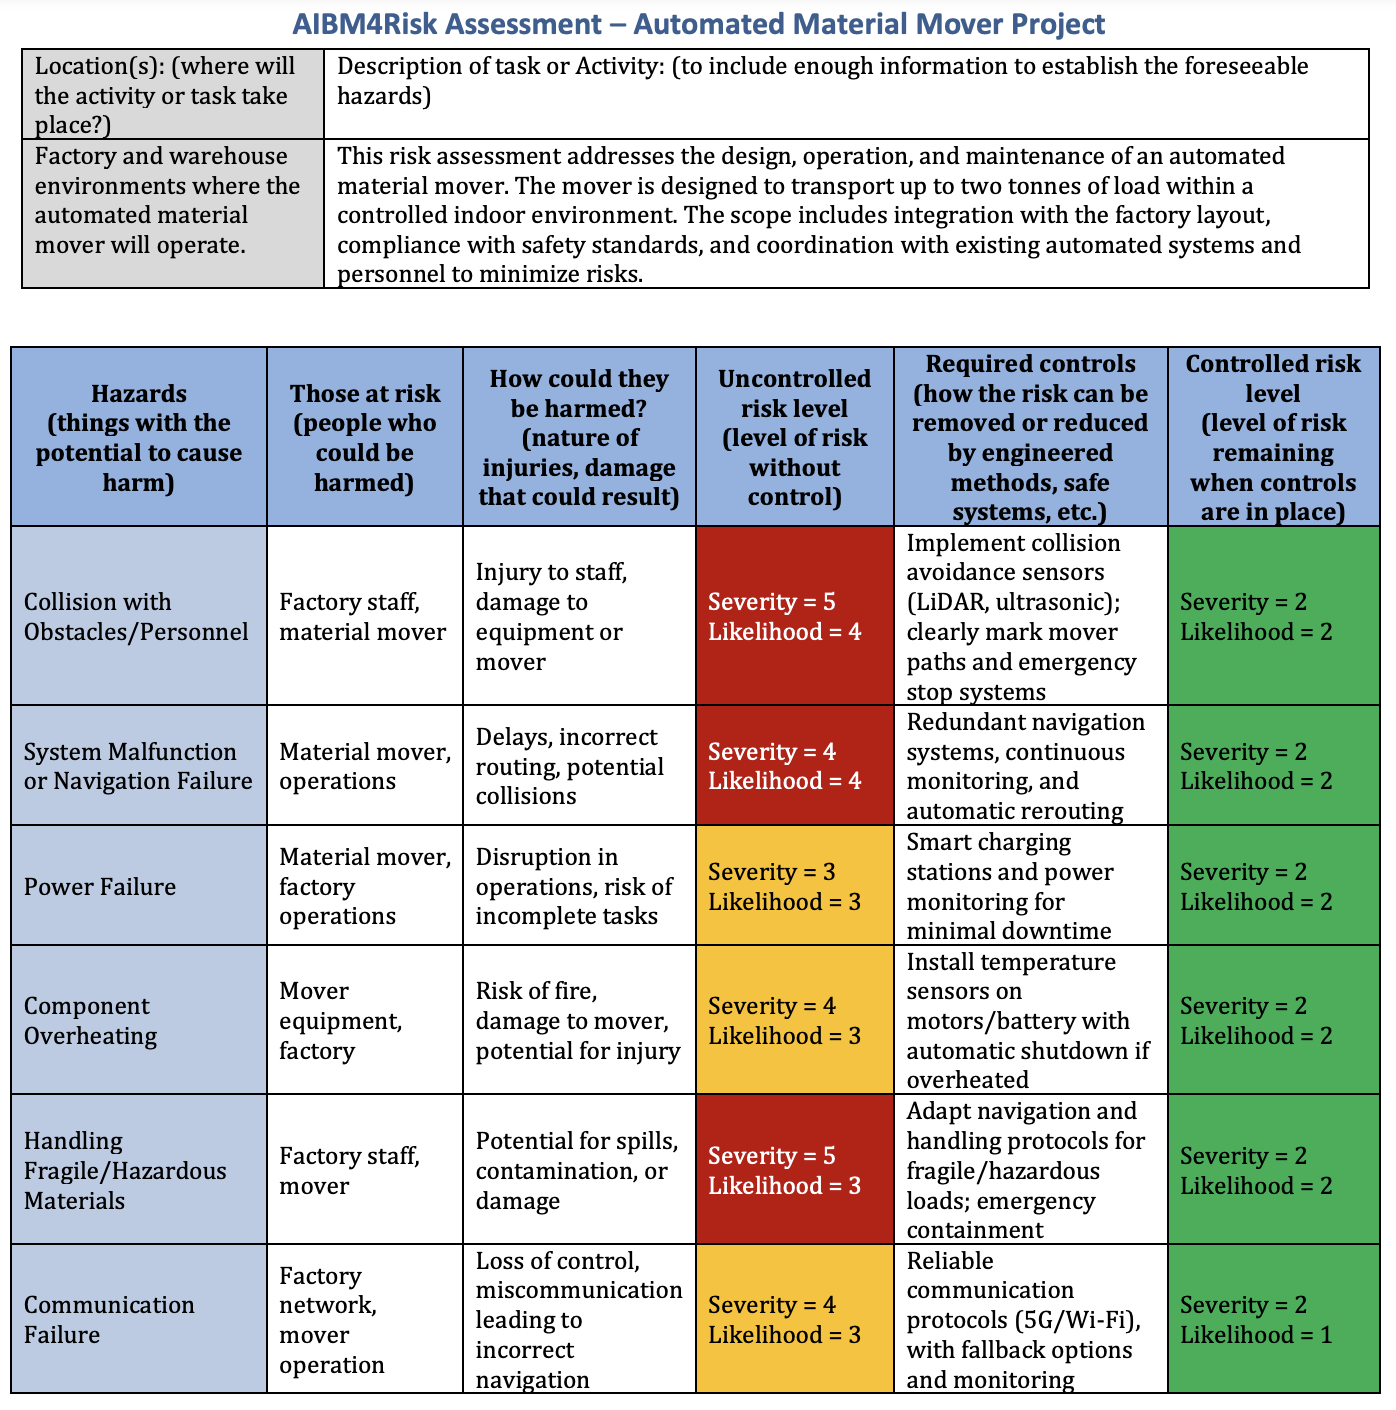
\includegraphics[width=0.7\textwidth]{Risk_Assessment_Automated_Material_Mover_Project1.png}
     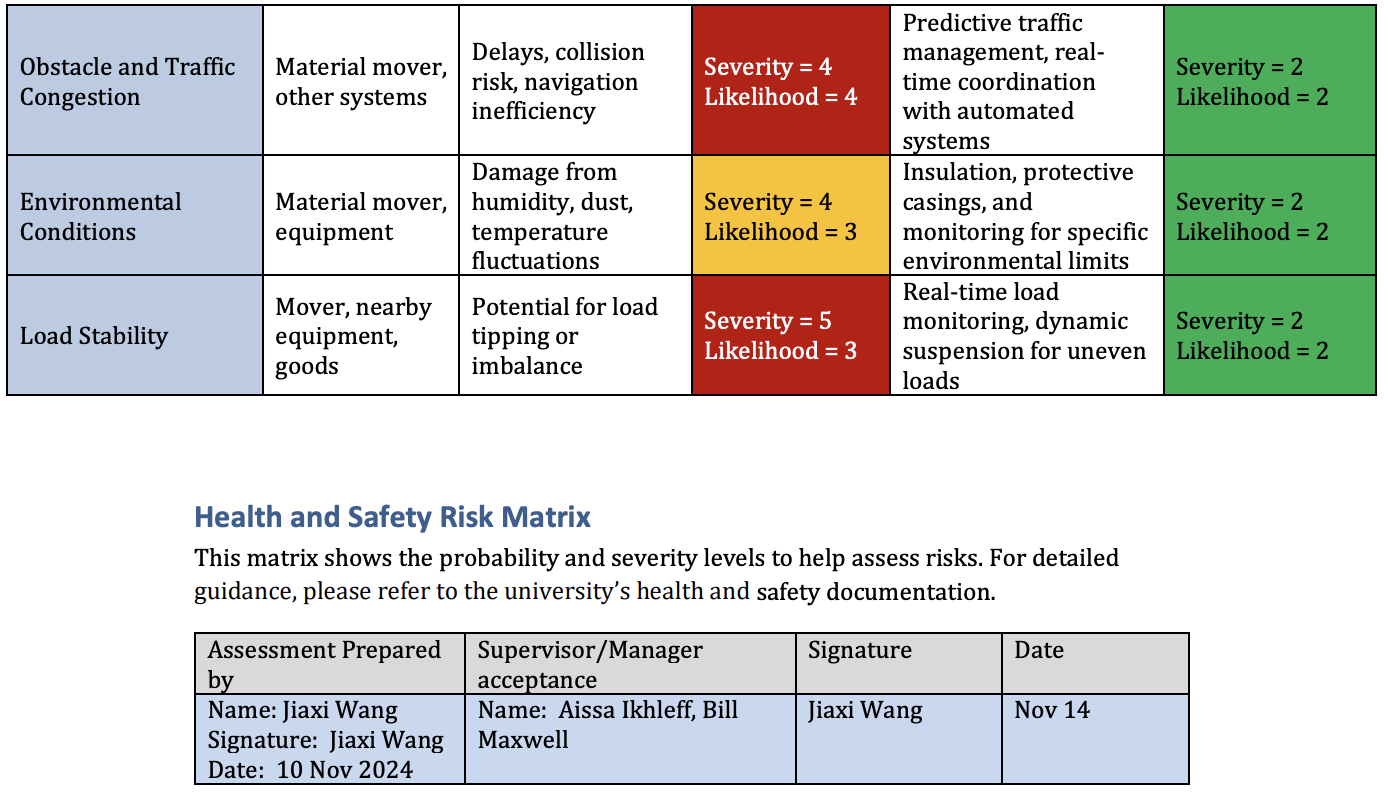
\includegraphics[width=0.7\textwidth]{Risk_Assessment_Automated_Material_Mover_Project2.png}
    \caption{Risk Assessment – Automated Material Mover Project}
    \label{fig:risk_assessment}
\end{figure}

\newpage



\section{Conclusion and Recommendations}
\begin{itemize}
    \item Modify the User Requirement Specification based on insights.
    \item Proceed with the project development.
    \item Aim for a 2-year ROI model to appeal to cost-sensitive customers.
\end{itemize}

\section{References}
Include citations and references here.

\section{Appendices}
Additional charts, data, or images can be appended here.

\end{document}
